\Lecture{Jayalal Sarma}{ 16 November, 2020}{32}{Incidence Algebra and Mobius Inversion Over Posets}{Kaushik Arcot}{$\alpha$}{JS}

\section{Recall}

\begin{theorem}[Stronger PIE]
  \label{stronger PIE}
  Let $f,g:2^{[n]}\longrightarrow \mathbb{R}$ are functions assigning real numbers to subsets of $[n]$ with the property that for any $A\subseteq [n]$

  \[ g(A)=\sum_{S\subseteq A} f(S)\]

  Then,
  \[ f(A) = \sum_{S \subseteq A} (-1)^{|A|-|S|}g(S)\]

\end{theorem}

\textbf{Mobius Inversion of Functions}

$f,g:\mathbb{N} \to \mathbb{R} ~satisfying,$ $\forall n ~g(n) = \sum_{d|n} f(d)  ~~then,$  
$$\forall n ~f(n) = \sum_{d|n} \mu(d)g(\frac{n}{d})$$

	\[
	\mu(d) = \begin{cases} 
	+1 , & ~if~ ~d~ ~is~ ~a~ ~\href{https://en.wikipedia.org/wiki/Square-free_integer}{square-free} ~positive~ ~integer~ ~with~ ~an~ ~even~ ~number~ ~of~ ~prime~ ~factors~~\\
 	-1 , & ~if~ ~d~ ~is~ ~a~ ~square-free~ ~positive~ ~integer~ ~with~ ~an~ ~odd~ ~number~ ~of~ ~prime~ ~factors~~\\
	0 , & otherwise
	\end{cases}
	\]

We can see in both cases that, there is an underlying poset for both the functions. For the first pair of functions, the poset is the Subset Poset, and for the second, it is the divisibilty poset. Our endeavour in this lecture is to further abstract this concept to any poset and acquire tools for algebra within poset functions, and then for Mobius Inversion of functions over posets.

\section{Incidence Algebra of Posets}

Let $P = (X,\le)$ be a poset. Let 

$$ A(P) = \{ f: X \times X \to \mathbb{R} | f(x,y) = 0, \forall x,y \in X  s.t x || y \}$$

Here $x || y$, indicates that x is incomparable to y in the Poset P. \\

Example functions : \\

\textbf{Zero Function} 

$$ O(x,y) = 0 \forall x,y \in X $$

\textbf{Kronecker Delta Function}

$$ \delta(x,y) =  \begin{cases} 
	1 , &  ~if~ ~x~ ~=~ ~y~ \\
	0 , & otherwise
	\end{cases} $$

\textbf{Characteristic Function of Poset}

$$ \zeta(x,y) =  \begin{cases} 
	1 , &  ~if~ ~x~ ~\le~ ~y~ \\
	0 , & otherwise
	\end{cases} $$

\medskip

\textbf{Addition Operator}

Given $f \in A(P)$ , $g \in A(P)$, the '+' operator

$$ (f+g) (x,y) = f(x,y) + g(x,y) $$

If $x || y$, then $f(x,y) = 0$, $g(x,y) = 0$, and hence $(f+g)(x,y) = 0$.
Thus $(f+g) \in A(P)$

\textbf{Remark} : A(P) forms a group with '+' operator as addition.

\medskip
\textbf{Scalar Multiplication}

Given $f \in A(P)$ , $c \in \mathbb{R}$,
$$ (cf)(x,y) = c*f(x,y)$$

If $x||y$, then $f(x,y) = 0$, and so $(cf)(x,y) = 0 $, Hence $(cf) \in A(P)$

\textbf{Remark} : $A(P)$ is closed under addition and scalar multiplication. Thus, $A(P)$ forms a vector space.

\medskip

\textbf{Convolution Operator}

We define the operator '*' over $A(P)$. Given two functions, 
$f,g \in A(P)$, the convolution operator is defined as,

$$ (f*g)(x,y) = \begin{cases} 
	\sum_{z:x\le z \le y} f(x,z)g(z,y), &  ~if~ ~x~ ~\le~ ~y~ \\
	0 , & otherwise
	\end{cases} $$
	
We find if  the following properties of the convolution operator hold or not.

\textbf{Commutative} \\

Convolution operator is not commutative. Assume $x,y \in X$ , such that $x \le y$ and there exists no such z such that $x \le z \le y$. Then,

$$ (f*g)(x,y) = f(x,x)g(x,y) + f(x,y)g(y,y)$$

$$ (g*f)(x,y) = g(x,x)f(x,y) + g(x,y)f(y,y)$$

These two expressions are not always equal. Assume $f(x,x) = 1$, $g(x,y) = 1$, and $f(x,y) = f(y,y) = 0$, $g(x,x) = g(y,y) = 0$. Then, we have

 $(f*g)(x,y) = 1$ and $(g*f)(x,y) = 0$. Therefore, convolution is not commutative.
 
\textbf{Associative}\\

The convolution operator is associative. To prove, assume $f,g,h \in A(P)$. Then,

$$((f*g)*h)(x, y) = \sum_{z: x \le z \le y}(f*g)(x, z) h(z, y)$$

$$ = \sum_{z: x \le z \le y}(\sum_{w: x \le w \le z}f(x, w)g(w, z))h(z, y)$$

By changing the order of the summations, we get,

$$ \sum_{w: x \le w \le z}f(x, w)(\sum_{z : w \le z \le y}g(w, z)h(z, y))$$

$$ = \sum_{w: x \le w \le z}f(x, w) (g*h)(w,y) $$

$$ = (f*(g*h)) (x,y)$$

Hence, convolution is associative.


\textbf{Identity}

\textbf{Claim} : The Kronecker Delta function is the identity function of A(P)

\begin{proof}
For $f \in A(P)$, if $x \le y$,
$$ (f*\delta)(x,y) = \sum_{z:x\le z \le y} f(x,z)\delta(z,y)$$
$$ =  \sum_{z:x\le z < y} f(x,z)\delta(z,y) + f(x,y)\delta(y,y)$$

Given that $z \ne y$, we have $\delta(z,y) = 0$. Thus, $(f*\delta)(x,y)$

$$ = f(x,y)\delta(y,y)$$

$\delta(y,y) = 1$, So

$$ = f(x,y) $$ 

Thus, Kronecker Delta function($\delta$) is the identity function of A(P).

\end{proof}

\section{Inverse of a Function}

The inverse of a function $f \in A(P)$, is a function $g$, such that

$$ (f*g)(x,y) = \delta(x,y)$$

Does the inverse of any $f \in A(P)$ exist ? No. In fact, we check for O(x,y). Let us assume there exists an inverse, Q(x,y) for the zero function. Then,
$$ (O*Q)(x,x) = \sum_{z:x\le z \le x} O(x,z)Q(z,x)$$

$$ = O(x,x)Q(x,x) = 0$$

But $\delta(x,x)$ = 1. Thus, O(x) (zero function) does not have an inverse. Can inverse exist for any other functions ? Yes, we see from this argument that for inverse to exist for $f \in A(P)$, there exists no $x \in X$, such that $f(x,x) = 0$. Infact, we prove next that for $f \in A(P)$, such that $\forall x \in X, f(x,x) \ne 0$, then there exists a unique inverse of f.

\section{Mobius Inversion over Posets}


\begin{lemma}
For any $f \in \mathbb{A}(P)$ such that $\forall x \in X, f(x,x) \ne 0$, there exists $g \in \mathbb{A}(P)$ (which we will call $f^{-1}$) such that $\forall x,y \in X, g \star f = \delta$ where $\delta$ is the Kronecker delta function.
\end{lemma}
\begin{proof}
We will directly write down the function $g$ based on $f$. For incomparable pairs $(x,y)$ we can define $g(x,y) = 0$. This ensures that $g \in \mathbb{A}(P)$. 

For comparable pairs, the function $g$ on input $(x,y)$ is defined based on an induction on a parameter of $\ell(x,y) \in X$. The distance between $x$ and $y$, denoted by $\ell(x,y)$ is said to be $k$, if $\exists z_1, z_2, \ldots z_{k-1}$ such that $x < z_1 < z_2 < \ldots < z_{k-1} < y$ and $\not\exists w_1, w_2, \ldots w_k$ such that $x < w_1 < w_2 < \ldots < w_{k-1} < w_k < y$. In other words, this is the length of the longest directed path from $x$ to $y$ (or vice versa).

Now we are ready to describe the definition of $g$ on comparable pairs $(x,y)$. 

As the base case, when $\ell(x,y) = 0$, we know that, $x=y$, hence we define:

$$g(x,x) = \frac{1}{f(x,x)}$$
Let us quickly check that this indeed satisfies the property that we wanted for inputs of the kind $(x,x)$. That is,
$$(g \star f) (x,x) = \sum_{x \le z \le y} g(x,z)f(z,y) = g(x,x)f(x,x) = 1 = \delta(x,x)$$

To do the definition inductively: let us assume that $g(x,y)$ is defined when $\ell(x,y) \le k$, and we consider a pair $(x,y)$ with distance $k+1$. We define :
$$g(x,y) = \frac{-1}{f(y,y)}\sum_{x \le z < y} g(x,z)f(z,y)$$
Note that this is well-defined since $g(x,z)$ is used in the RHS only for pairs $(x,z)$ with $\ell(x,z) \le k$ and that $f(y,y) \ne 0$ for every $y \in X$.
With this definition :
\begin{eqnarray*}
(g \star f) (x,y) & = & \sum_{x \le z \le y} g(x,z)f(z,y)\\
& = & \sum_{x \le z < y} g(x,z)f(z,y) + g(x,y)f(y,y)\\
& = & \sum_{x \le z < y} g(x,z)f(z,y) + \left(\frac{-1}{f(y,y)}\sum_{x \le z < y} g(x,z)f(z,y)\right) f(y,y) \\
& = & 0 = \delta(x,y)
\end{eqnarray*}
Since $g \in \mathbb{A}(P)$ we have completed the proof.
\end{proof}


\Lecture{Jayalal Sarma}{ 18 November, 2020}{33}{Mobius Inversion Theorem for Posets and Corollaries}{Abhishek Aladahalli}{$\alpha$}{JS}

\noindent In particular the \textbf{zeta function} ($\zeta$)
$$ \zeta (x, y) =  
\begin{cases}
&1 ~~~~\textrm{if} ~~x \le y \\
&0 ~~~~\textrm{otherwise} \\
\end{cases}
$$
has an inverse called the \textbf{Mobius Function} ($\mu$) of the poset.\\

\noindent From the lemma proved above we define Mobius Function as,

\noindent \underline{For $x = y$},
$$g(x,x) = \mu(x,x) = \frac{1}{\zeta (x,x)} = 1$$
$$=> \boxed{\mu(x,x) = 1 ~~ (\textrm{Since} ~\zeta (x,x) = 1)}$$

\noindent \underline{For $x ~ || ~ y$}, (i.e. when $x$ and $y$ are incomparable)
$$g(x,y) = \mu(x,y) = \frac{-1}{\zeta(y,y)}\sum_{x \le z < y} \mu(x,z) \zeta(z,y)$$
$$=> \mu(x,y) = -1\sum_{x \le z < y} \mu(x,z) \zeta(z,y) $$
$$=> \mu(x,y) = -1\sum_{x \le z < y} \mu(x,z) (0) $$
(Since, zeta function ($\zeta$) is $0$ for $x$ and $y$ which are incomparable)
$$=> \boxed{\mu(x,y) = 0}$$

\noindent \underline{For $x \le y$},
$$g(x,y) = \mu(x,y) = \frac{-1}{\zeta(y,y)}\sum_{x \le z < y} \mu(x,z) \zeta(z,y)$$
$$=> \mu(x,y) = -1\sum_{x \le z < y} \mu(x,z) \zeta(z,y) $$
$$=> \mu(x,y) = -1\sum_{x \le z < y} \mu(x,z) (1) ~~~~(\textrm{Since}~~ \zeta(z,y) = 1 ~ \textrm{for} ~z < y)$$
$$=> \boxed{\mu(x,y) = -\sum_{x \le z < y} \mu(x,z)}$$

Hence, Mobius Function is defined as

\begin{center}
    \doublebox{ $\mu (x, y) =  
    \begin{cases}
    &-\sum\limits_{x \le z < y} \mu(x,z) ~~~~~~~~~~~~~~~~~~~~~\textrm{if} ~~x < y \\
    &1 ~~~~~~~~~~~~~~~~~~~~~~~~~~~~~~~~~~~~~~~~~~~~~\textrm{if} ~~ x=y \\
    &0 ~~~~~~~~~~~~~~~~~~~~~~~~~~~~~~~~~~~~~~~~~~~~~\textrm{if x and y are incomparable i.e.} ~~ x ~||~ y\\
    \end{cases}$ }
\end{center}


\noindent Now, Let's consider an example of Divisibility Poset and apply the mobius function on it, 

\begin{center}

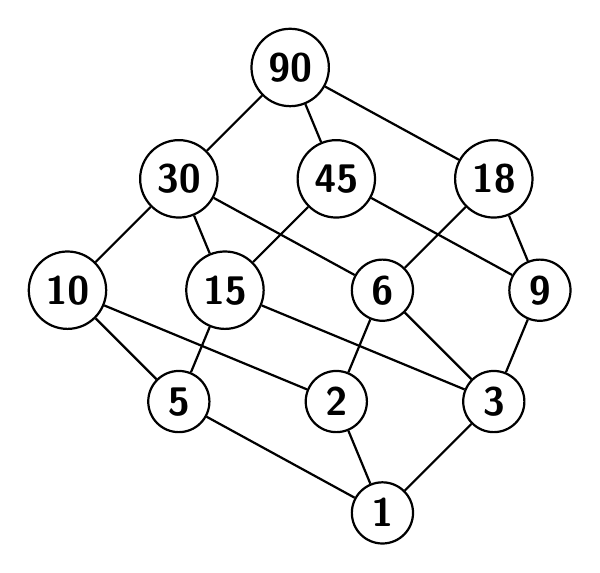
\begin{tikzpicture}[auto, node distance=2cm, every loop/.style={}, thick,main node/.style={circle,draw,font=\sffamily\Large\bfseries}]

\node[main node] (1) {90};
\node[main node] (2) [below left of=1] {30};
\node[main node] (3) [right of=2] {45};
\node[main node] (4) [right of=3] {18};
\node[main node] (5) [below left of=2] {10};
\node[main node] (6) [right of=5] {15};
\node[main node] (7) [right of=6] {6};
\node[main node] (8) [right of=7] {9};
\node[main node] (9) [below right of=5] {5};
\node[main node] (10) [right of=9] {2};
\node[main node] (11) [right of=10] {3};
\node[main node] (12) [below left of=11] {1};


\path[every node/.style={font=\sffamily\small}]
    (1) edge node [] {} (4)
        edge node [] {} (3)
        edge node [] {} (2)
    (2) edge node [] {} (5)
        edge node [] {} (6)
        edge node [] {} (7)
    (3) edge node [] {} (6)
        edge node [] {} (8)
    (4) edge node [] {} (7)
        edge node [] {} (8)
    (5) edge node [] {} (9)
        edge node [] {} (10)
    (6) edge node [] {} (9)
        edge node [] {} (11)
    (7) edge node [] {} (10)
        edge node [] {} (11)
    (8) edge node [] {} (11)
    (9) edge node [] {} (12)
    (10) edge node [] {} (12)
    (11) edge node [] {} (12);

\end{tikzpicture}
    
\end{center}

\begin{align*}
\textrm{For} ~~(x,y) = (1,1),\\
    \mu (x,y) &= \mu (1,1)\\
=>  \mu (1,1) &= 1~~~~~~~~~~~(\because x = y)\\\\
\textrm{For} ~~(x,y) = (1,2),\\
    \mu (x,y) &= \mu (1,2)\\
=>  \mu (1,2) &= -\sum\limits_{1 \le z < 2} \mu(1,z)    ~~~~~~~\textrm{(By definition of mobius function)}\\
    &= - \mu(1,1)\\
=>  \mu(1,2) &= -1\\\\
\textrm{Similarly for} ~~(x,y) = (1,3),\\
=> \mu(1,3) &= -1\\\\
\textrm{Similarly for} ~~(x,y) = (1,5),\\
=> \mu(1,5) &= -1\\
\end{align*}

Thus, In general for a prime number $p$,

\begin{center}
    \doublebox{
    $\mu(1,p) = -1$
    }
\end{center}

Now,
\begin{align*}
\textrm{For} ~~(x,y) = (1,10),\\
    \mu (x,y) &= \mu (1,10)\\
=>  \mu (1,10) &= -\sum\limits_{1 \le z < 10} \mu(1,z)    ~~~~~~~\textrm{(By definition of mobius function)}\\
    &= - (\mu(1,1) + \mu(1,2) + \mu(1,5)) \\
=>  \mu(1,10) &= 1\\\\
\textrm{Similarly for} ~~(x,y) = (1,15),\\
=> \mu(1,15) &= 1\\\\
\textrm{Similarly for} ~~(x,y) = (1,6),\\
=> \mu(1,6) &= 1\\
\end{align*}

Thus, In general for prime numbers $p$ and $q$ ,
\begin{center}
    $\mu(1,p q) = -(\mu(1,1) + \mu(1,p) + \mu(1,q))$\\
    $=>$\doublebox{
    $\mu(1,p q) = 1$
    }
\end{center}

\noindent Now,
\begin{align*}
\textrm{For} ~~(x,y) = (1,9),\\
    \mu (x,y) &= \mu (1,9)\\
=>  \mu (1,9) &= -\sum\limits_{1 \le z < 9} \mu(1,z)    ~~~~~~~\textrm{(By definition of mobius function)}\\
    &= - (\mu(1,1) + \mu(1,3)) \\
=>  \mu(1,9) &= 0\\
\end{align*}

Thus, In general for a prime number $p$,

\begin{center}
    \doublebox{
    $\mu(1,p^2) = 0$
    }
\end{center}

\noindent Now,
\begin{align*}
\textrm{For} ~~(x,y) = (1,45),\\
    \mu (x,y) &= \mu (1,45)\\
=>  \mu (1,45) &= -\sum\limits_{1 \le z < 45} \mu(1,z)    ~~~~~~~\textrm{(By definition of mobius function)}\\
    &= - (\mu(1,1) + \mu(1,3) + \mu(1,5) + \mu(1,9) + \mu(1,15)) \\
=>  \mu(1,45) &= 0\\\\
\textrm{Similarly for} ~~(x,y) = (1,18),\\
=> \mu(1,18) &= 0\\
\end{align*}

Thus, In general for prime numbers $p$ and $q$,

\begin{center}
    $\mu(1,p^2 q) = -(\mu(1,1) + \mu(1,p) + \mu(1,q) + \mu(1,p q) + \mu(1,p^2) )$
    \\
    $=>$\doublebox{
    $\mu(1,p^2 q) = 0$
    }
\end{center}

\noindent Now,
\begin{align*}
\textrm{For} ~~(x,y) = (1,30),\\
    \mu (x,y) &= \mu (1,30)\\
=>  \mu (1,30) &= -\sum\limits_{1 \le z < 30} \mu(1,z)    ~~~~~~~\textrm{(By definition of mobius function)}\\
    &= - (\mu(1,1) + \mu(1,3) + \mu(1,5) + \mu(1,2) + \mu(1,6) + \mu(1,10) + \mu(1,15)) \\
=>  \mu(1,30) &= -1\\
\end{align*}

Thus, In general for prime numbers $p$, $q$ and $r$,

\begin{center}
    $\mu(1,p q r) = -(\mu(1,1) + \mu(1,p) + \mu(1,q) + \mu(1,p q) + \mu(1,q r) + \mu (1, p r) )$
    \\
    \doublebox{
    $\mu(1,p q r) = 1$
    }
\end{center}

Therefore In general, The mobius function for the divisibility poset turns out to be,

\begin{center}
    \doublebox{ $\mu (d)
    \begin{cases}
        &= +1 ~~~~~~~~~~~~\textrm{If $d$ is a product of even number of primes}\\
        &= -1 ~~~~~~~~~~~~\textrm{If $d$ is a product of odd number of primes}\\
        &= 0 ~~~~~~~~~~~~~\textrm{Otherwise}\\
    \end{cases}
    $
    }
\end{center}

\section{Mobius Inversion theorem over Posets}

\textbf{Assumption :}

\noindent In the poset $X$, there is a unique $m$ such that $\forall x \in X$, $m \le x$

\begin{theorem}

For a poset $X$, if $f$ is a function $f: X \rightarrow \mathbb{R}$ and $g$ is a function $g: X \rightarrow \mathbb{R}$ such that,
$$\forall a \in X, ~~~~~~~~g(a) = \sum_{x \le a} f(x)$$ 
then
$$\boxed{\forall a \in X, ~~~~~~~~f(a) = \sum_{x \le a} \mu(x,a) g(x)}$$
where $\mu$ is the mobius function of the poset.
\end{theorem}

\begin{proof}

As from the assumption, let $m$ be the unique minimal element of the poset $X$.

\noindent And let $f$ and $g$ be the functions defined as above such that 

$$\forall a \in X, ~~g(a) = \sum\limits_{x \le a} f(x)  ~~~~~~~~~(1)$$

\noindent Now, we define two functions $F(x,y)$ and $G(x,y)$ such that,

\begin{Parallel}[v]{0.48\textwidth}{0.48\textwidth}
\ParallelLText{
\begin{align*}
   & \forall a \in X ,\\
   & F(m,a) = f(a)\\
   & G(m,a) = g(a)\\
\end{align*}}
\ParallelRText{
\begin{align*}
   & \textrm{For all other}~ x ~\textrm{and} ~ y ~ \textrm{where} ~ x \ne m,\\
   & F(x,y) = 0\\
   & G(x,y) = 0\\
\end{align*}
}
  \ParallelPar
\end{Parallel}

\noindent Thus, By Incidence Algebra $F,G \in A(P)$ for $P(X,\le)$.\\

\noindent \textbf{Claim :}
$$\boxed{G = F \star \zeta ~~\textrm{where $\zeta$ is the zeta function.}}$$

\noindent \underline{Note:} Through this claim we can show that $F = G \star \mu$ (where $\mu$ is the mobius function) and thus proving the theorem.\\


\noindent \textbf{Proof for the claim :}

\noindent Consider $G(x,y)$,

\textbf{Case 1 : $\forall a \in X$}
\begin{align*}
    G(m,a) &= g(a)\\
    &= \sum_{x \le a} f(x) ~~~~~~~~~~~~~~~~ \textrm{( $\because~$ from (1))}\\
    &= \sum_{m \le x \le a} F(m,x) ~~~~~~~~ \textrm{($\because~$from definition of $F(x,y)$)}\\
    &= \sum_{m \le x \le a} F(m,x) \zeta(x,a) ~~~~~~\textrm{($\because \zeta (x,a) = 1, \forall x \le a$ )}
\end{align*}
$$=> \boxed{G(m,a) = F \star \zeta (m,a)} ~~~~~~~~~~~~ \textrm{( $\because~$ By defintion of convolution ($\star$))}$$

\textbf{Case 2 :} For all other $x$ and $y$ where $x \ne m$
\begin{align*}
    G(x,y) &= 0\\
    &= \sum_{x \le z \le y} F(x,z) \zeta(z,y) ~~~~~~\textrm{($\because F(x,z) = 0, \forall x \ne m$ )}
\end{align*}
$$=> \boxed{G(x,y) = F \star \zeta (x,y)} ~~~~~~~~~~~~ \textrm{($\because~$By defintion of convolution ($\star$))}$$

\noindent Hence, The claim $G = F \star \zeta $ is true.\\

\noindent Thus, By definition
$$\boxed{F = G \star \mu}$$

\noindent Therefore, $\forall a \in X$,
\begin{align*}
    F(m,a) &= \sum_{m \le x \le a} G(m,x) \mu(x,a) ~~~~~~~~ \textrm{($\because~$By defintion of convolution ($\star$))}\\
 => f(a)  &=\sum_{x \le a} g(x) \mu(x,a) ~~~~~~~~ \textrm{($\because~$From defintion of $F(m,a) = f(a), G(m,x) = g(x)$)}
\end{align*}

\noindent Thus,
\begin{center}
    \doublebox{$\forall a \in X, ~~~~~~~~f(a)  = \sum\limits_{x \le a} \mu(x,a) g(x)$}
\end{center}

Hence Proved.\\

\end{proof}

\subsection{Corollary}

\noindent \underline{\textbf{Application of Mobius Inversion theorem on Subset Poset}}\\

\noindent For the subset poset we will show, if $f$ and $g$ are functions defined from subsets to real numbers (i.e. 
$f: 2^{[n]} \rightarrow \R$ , $g: 2^{[n]} \rightarrow \R $ ) such that
$$\forall A \subseteq [n], ~~~~~ g(A) = \sum_{S \subseteq A} f(S) $$
then
$$\boxed{\forall A \subseteq [n], ~~~~~ f(A) = \sum_{S \subseteq A} (-1)^{|A|- |S|}g(S) } $$

\noindent \textbf{Claim :} For $X \subseteq [n]$ and $Y \subseteq [n]$,
$$ \mu (X,Y) = 
\begin{cases}
    &0 ~~~~~~~~~~~~~~~~~~~~~~~~~~~~\textrm{if $~X \nsubseteq Y$}\\
    &(-1)^{|Y| - |X|} ~~~~~~~~~~\textrm{if $~X \subseteq Y$}\\
\end{cases}
$$
\underline{\textsf{Note :}} If we prove the claim to be true then the above subset poset can directly be shown as a corollary of the mobius inversion theorem by substituting the value of $\mu$.\\

\noindent \textbf{Proof for the claim :} 

\noindent We will apply Induction on $|Y|-|X|$ for $X \subseteq Y$.\\

\noindent \underline{Base step}, For $|Y| - |X| = 0$ i.e. $X = Y$
\begin{align*}
    \mu (X,Y) &= \mu(X,X)\\
    => \mu (X,Y) &= 1  ~~~~~~~~~~\textrm{($\because X \subseteq X ~$ and $~\mu (X,X) = 1$ )}\\
    => \mu (X,Y) &= (-1)^{0} = (-1)^{|Y| - |X|}
\end{align*}

\noindent \underline{Induction step}, Assume it's true for $|Y| - |X| \le k$. Now, we need to prove it's also true for $|Y| - |X| = k + 1$.\\

\noindent Thus, Consider $\mu (X,Y)$ for $|Y| - |X| = k + 1$,
\begin{align*}
    \mu (X,Y) &= - \sum_{X \subseteq Z \subset Y} \mu (X,Z) ~~~~~~~~~~~~~\textrm{($\because X < Y~$ and by definition of mobius function )}\\
 => \mu (X,Y) &= - \sum_{X \subseteq Z \subset Y} (-1)^{|Z|-|X|} ~~~~~~~\textrm{($\because |Z| - |X| \le k~$ and it's assumed true for $|Y| - |X| \le k$)}\\
 => \mu (X,Y) &= - \sum_{X \subseteq Z \subseteq Y} (-1)^{|Z|-|X|} + (-1)^{|Y| - |X|} ~~~~~~~\textrm{($\because~$Adding and subtracting the subset $Y$)}
\end{align*}
$$=> \boxed{\mu (X,Y) = - \sum_{X \subseteq Z \subseteq Y} (-1)^{|Z|-|X|} + (-1)^{|Y| - |X|}} ~~~~~~\textrm{(1)}$$

\noindent Now, we will show that 1st term in the R.H.S goes to 0 by using a combinatorial argument.\\

\noindent So, For given $X, Y \subseteq [n]$ and $X \subseteq Y$,
\begin{align*}
    \sum_{X \subseteq Z \subseteq Y} (-1)^{|Z|-|X|} &= \sum_{k} \sum_{\substack{X \subseteq Z \subseteq Y\\ |Z| - |X| = k}} (-1)^k ~~~~~\textrm{(By rewriting the summation based on the size of $|Z| - |X|$)}\\
    &= \sum_{k} (-1)^k {n \choose k} ~~~~~~~~~\textrm{($\because~$ Number of ways of choosing such a subset $|Z|$ is ${n \choose k}$) }\\
    &= 0 ~~~~~~~~~~~~~~~~~~~~~~~~~~\textrm{($\because ~$ Signed summation of binomial coefficients is $0$)}\\
=> \sum_{X \subseteq Z \subseteq Y} (-1)^{|Z|-|X|} &= 0\\
\end{align*}
Therefore, Equation (1) becomes,\\

\begin{center}
    \doublebox{
$\mu (X,Y) = (-1)^{|Y|-|X|}$
}
\end{center}

Hence Proved.\\

\noindent Thus, from this definition of $\mu$ and the theorem of Mobius Inversion, the corollary on the subset poset follows that ,\\

\noindent \textbf{Corollary :} If $f$ and $g$ are functions defined from subsets to real numbers (i.e. 
$f: 2^{[n]} \rightarrow \R$ , $g: 2^{[n]} \rightarrow \R $ ) such that
$$\forall A \subseteq [n], ~~~~~ g(A) = \sum_{S \subseteq A} f(S) $$
then
\begin{center}
    \doublebox{
    $\forall A \subseteq [n], ~~~~~ f(A) = \sum\limits_{S \subseteq A} (-1)^{|A|- |S|}g(S) $
    }
\end{center}











\Lecture{Jayalal Sarma}{ 19 November, 2020}{34}{More Applications of Structure of Partial Orders, Fixed Point Theorems}{Kaushik Arcot, Abhishek Aladahalli}{$\alpha$}{JS}

\section{Equinumerous Sets and Bijections}

We define Cardinality using the concept of Bijections and Equinumerous sets.
\begin{theorem}
Two sets A, B are equinumerous or equal in cardinality iff there
exists a bijection $f: A \to B$. Or,\\

$ |A| = |B| \Leftrightarrow \exists$ bijection $f:A \to B $ \\

\end{theorem}

\textbf{Example of Equinumerous sets and Bijections}\\

\textbf{Even Numbers and $\mathbb{N}$}\\

$f:\mathbb{E} \to \mathbb{N}$,  $f(x) = x/2$

Is a bijection from even numbers to Natural Numbers.\\

The Noton of Cardinality arises from the fact that these Equinumerous sets divide the Subset Partial Order into different equivalence classes and each of those classes correspond to different cardinalities. \\

So to prove that two sets are equinumerous sets, we need to prove there exists a bijection between the two sets. To prove that there exists a bijection between two sets, we can just prove that there exists an injection in both directons.

\begin{theorem}[Cantor Schroeder Bernstein Theorem]
$A,B \subseteq U$ ,$\exists f:A \to B, g:B \to A$ are injections $\implies \exists h:A \to B$ which is a bijection 
\end{theorem}

This theorem is intuitive in finite sets, but to prove for infinite sets, we need some more tools that concern posets and cardinality.

\section{Knaster-Tarski Fixed point theorem}

To prove this theorem, we need to understand some properties.

\textbf{Fixed Point of a Function}\\
Let $f: X \to X$, be a function. Then, a point $x \in X$, is said to be a fixed point of function $f$ if $f(x) = x$.

\textbf{Preserving Order of Posets}

Let $P(X,\le)$ be a poset. Then any function $f: X \to X$ is said to preserve order if 
$$ \forall x,y \in X, x \le y \implies f(x)  \le f(y) $$

\textbf{Upper Bound of a Set}

Let $P(X,\le)$ be a poset, and $A \subseteq X$, then the upper bound of set A is defined as 

$$ UB(A) = \{x \in X | \forall y \in A, y \le x\} $$

\textbf{Least Upper Bound of a Set}

Let $P(X,\le)$ be a poset, and $A \subseteq X$, then the least upper bound of set A is defined from the upper bound set, as the least element in the upper bound set of A.

$$ LUB(A) = \{x  | \forall y \in UB(A), x \le y\} $$

\textbf{Complete Partial Order}

A partial order $P(X,\le)$ is set to be a complete partial order, if $\forall A \subseteq X$ , $\exists LUB(A)$

\medskip


We can understand the notion of a complete partial order using the subsets partial order. Let $P(X,\le)$, be the subsets partial order, where $X = 2^{[n]}$. Then, let $A \subseteq X$, be a subset of X, which is a set of subsets of $[n]$. Assume, $A = \{A_1,A_2,...A_k\}$, and S =  $\bigcup_{i=1}^{k} A_{i}$ forms the LUB of the set A. We know that $\forall i \in [k], A_i \le S$, (because $A_i$ is a subset of S, S is the union of all $A_i$'s). And it is the lowest upper bound, as any element missing from $S$, will be present in one of the $A_i$'s.

Now, we're ready to prove the Knaster-Tarski Theorem.

\begin{theorem}[Knaster-Tarski Fixed point theorem]
Let $P(X,\le)$ be a complete partial order, and let $f: X \to X$, be a function that preserves the order on the partial order P. Then $f$ has a fixed point.
\end{theorem}

\begin{proof}
Consider the set $A = \{x | x \le f(x)\}$. Assume that A is non-empty. This is possible when X has a least element in P. Then, for that least element $x \in X$, $\forall y \in X, x \le y$. And $f(x) \in X$, thus, $x \le f(x)$, and therefore $x \in A$. \\

\textbf{Observation} If $x \in A$, then $f(x) \in A$. \\
$x \in A$. $\implies x \le f(x)$. As f preserves order,\\
$ \implies f(x) \le f(f(x) $. Let f(x) = z, then \\
$z \le f(z)$. Thus, $z \in A$. $\implies f(x) \in A$.\\

Since the partial order is complete, and $A \subseteq X$, there exists an LUB(A). Let

$$ y = LUB(A)$$

Consider, $\forall x \in A$. As y is LUB,\\
$x \le y$ , As f preserves order\\
$ f(x) \le f(y) $. Becasue $x \in A$, \\

$x \le f(x) \le f(y), \forall x \in A$ \\

This implies that $f(y)$ is an upper bound of A. Since $y$ is the LUB of A,
$$y \le f(y) $$

By the property of A, it is clear that $y \in A$. And because $y \in A$, and from the observation proven above, we have that $f(y) \in A$. \\

Since $f(y) \le A$, and y is LUB(A) of A, we have that
$$ f(y) \le y $$

So, we have,
$$ f(y) \le y \And y \le f(y) $$.

By the anti-symmetry of the relation $\le$ in the partial order, we have 
$$f(y) = y $$

So, we have $y$ as the fixed point.\\

Hence proved.

\end{proof}


\section{Cantor-Schroeder-Bernstein Theorem}

\begin{theorem}[Cantor Schroeder Bernstein Theorem]
$A,B \subseteq U$ ,$\exists f:A \to B, g:B \to A$ that are injections $\implies \exists h:A \to B$ which is a bijection.
\end{theorem}

\begin{proof}

We find a $H \subseteq A$, and we build a function h, such that
$$ h |_H = f \And h|_{\bar H} = g $$

Then, we prove that H is a bijection.

\textbf{Claim} For $H \subseteq A$, if $g( \bar{f(H)} ) = \bar H$ then by  the above definition, h is a bijection. \\

Or, we have to find an H such that $H = \bar{g(\bar{f(H)})}$ \\


First, we find an H such that this claim is satisfied, and then we prove the claim. \\

We define the following function on the subset partial order of A.\\

$\tau : 2^{[A]} \to 2^{[A]}$, such that for any $T \subset A$,

$$ \tau(T) = \bar{g(\bar{f(T)})}$$

We will prove the properties of preserving order and completeness of this Partial Order. \\

We know that the partial order is complete, as it is a subset poset. \\

For preserving order, assume $S \subset T$. . By applying f on both sides, we have $f(S) \subset f(T)$. \\

Taking complement, we have $\bar{f(T)} \subset \bar{f(S)}$.\\

As g is a function from B to A, and $f(x) \in B \forall x \in A$, applying g on both sides, we get \\

$$ g(\bar{f(T)}) \subset g(\bar{f(S)})$$

Again taking complement, we get 

$$ \bar{g(\bar{f(S)})} \subset \bar{g(\bar{f(T)})} $$

So, $\tau(S) \subset \tau(T)$. Hence $\tau$ preserves order.\\

Because $\tau$ preserves order and and $P = ([A],\le)$ is a complete poset, we have that there exists a fixed point for $\tau$. Therefore

$$ \exists H \subset A, \bar{g(\bar{f(H)})} = H $$

Now that we have arrived at an H, we now need to prove that $h$ is a bijection. We need to prove three parts. \\

\textbf{Well-defined} \\
h is well defined. $\forall x \in A$, if $x \in H$, the output of $h$ is f(x). Otherwise, as $g$ is injective, and $\bar H = g(\bar{f(H)})$, and so $\bar H \subseteq g(B)$, and $g^{-1}(x)$ is defined $\forall x \in g(B)$, and subsequently in $\bar H$. So $\forall x \in A$, h(x) is well defined.

\textbf{Injective}\\
We need to prove $\forall x,y \in A$, $x \ne y \implies h(x) \ne h(y)$.

\textsf{Case 1} : $x \in H \And y \in H$\\

$\forall x \in H$, $h(x) = f(x)$. Therefore, $x \ne y \implies f(x) \ne f(y) \implies h(x) \ne h(y) $


\textsf{Case 2}: $x \in \bar H \And y \in \bar H$

$\forall x \in \bar H$, $h(x) = g^{-1}(x)$.  Since g is injective, $g^{-1}$  is well-defined, and thus $g^{-1}(x) \ne g^{-1}(y) \implies h(x) \ne h(y)$

\textsf{Case 3} : $x \in H \And y \in \bar H$
For $x \in H$, $h(x) = f(x)$\\
For $y \in \bar H$, $h(y) = g^{-1}(y)$ \\

We need to prove $h(x) \ne g^{-1}(y)$ \\

We know, $g(\bar{f(H)}) = \bar H $. As $g^{-1}$ is well defined, $\implies g^{-1}(\bar H) \subseteq \bar{f(H)}$ \\. Therefore, $g^{-1}(H) \nsubseteq f(H)$. Moreover, as $g^{-1}(\bar H) \subseteq \bar{f(H)}$, $ \nexists u \in \bar H$, such that $g^{-1}(u) \in f(H)$.
Thus, for $x \in H \And y \in \bar H$, $g^{-1}(y) \ne f(x)$. Hence proved.

\textbf{Surjective} \\
To prove, $range(h) = B$. That is, $\forall y \in B, \exists x \in A$, such that $h(x) = y$. Assume, $y \in f(H)$. Given that $\forall x in H, h(x) = f(x)$, and because $y \in f(H)$, $\exists x, f(x) = y$.

Now, for $x \in \bar{f(H)}$. We know,

\begin{equation} \label{eqn:1} \bar H = g(\bar{f(H)}) \end{equation}

And that $g^{-1}(x)$ is defined $\forall x \in \bar H$ (already proved). Since $g^{-1}$ is obviously injective ( if $x \ne y$ and  $g^{-1}(x) = g^{-1}(y) = a$, then $g(a)$ is not defined), we can apply $g^{-1}$ on both sides of \ref{eqn:1}, to get 

$$ g^{-1}(\ba   r H) \subseteq \bar{f(H)}$$

As $g{-1}$ is injective, and we know that $|\bar H| = g(\bar{f(H)})$, both the sets are of the same size, thus,
$$ g^{-1}(\bar H) = \bar{f(H)}$$.

$\forall x \in \bar{f(H)}$, we have a pre-image in $g^{-1}(\bar H)$. Hence, h is surjective.

From the three parts, we have proven that $h : A \to B$, is a bijective function, constructed from $f : A \to B$ and $g : B \to A$, two injective functions.

\end{proof}
